% \documentclass[tikz]{standalone}
% \usepackage{pgfplots}
% \begin{document}
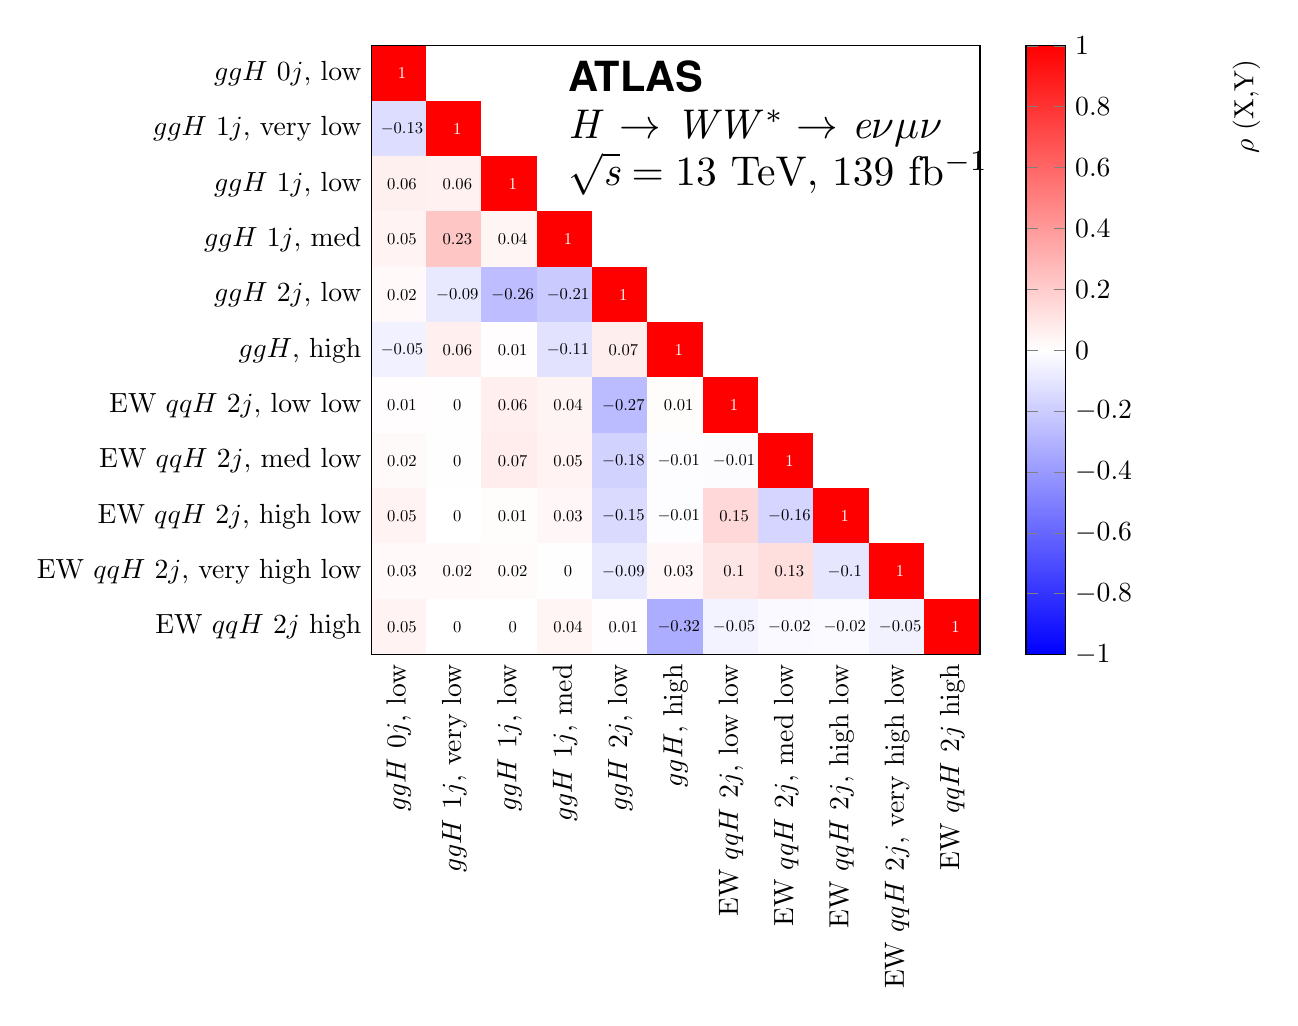
\begin{tikzpicture}
\begin{axis}[
    colormap={bluewhitered}{color=(blue) color=(white) color=(red)},
    clip=false,
    colorbar,
    colorbar style={
    ytick={-1,-0.8,...,1},
    ylabel={$\rho$ (X,Y)},
    ylabel style={
        at={(ticklabel cs:0.9)}
    },
    yticklabel style={
    text width=5em,
    ytick={-1,-0.8,...,1},
        tick style={draw=gray!}
        }
    },
    colormap name={bluewhitered},
   %  colormap/jet,
   % colorbar,
   % point meta min=0.0,
   % point meta max=0.2860,
   %  colorbar style={ height= 10 cm},xtick={0,0.286},
    % x=1em,
    % y=1em,
    x=2em,
    y=2em,
    xtick=data,
    ytick=data,
    ymin={$ggH~0j$, low \pTH},
    ymax={EW $qqH~2j$ high \pTH},
    xmin={$ggH~0j$, low \pTH},
    xmax={EW $qqH~2j$ high \pTH},
    y dir=reverse,
    % enlarge x limits={abs=0.5em},
    % enlarge y limits={abs=0.5em},
    enlarge x limits={abs=1em},
    enlarge y limits={abs=1em},
    point meta min=-1,
    point meta max=+1,
    % grid=both,
    major grid style={draw=none},
    visualization depends on={x\as\X},
    visualization depends on={y\as\Y},
    visualization depends on={correlations\as\Z},
    nodes near coords={\pgfmathtruncatemacro{\Z}
    {ifthenelse(\Y<\X,0,1)}
    \ifnum\Z=0
    \else\pgfmathprintnumber\pgfplotspointmeta\fi},
    % \ifthenelse{\X=+1}{\def\col{red}}{\def\col{black}},
    % every node near coord/.append style={anchor=center,scale=0.6,/pgf/number format/.cd,fixed,precision=2},
        % nodes near coord/.append={\pgfmathprintnumber\pgfplotspointmeta\,},
        % % ---------------------------------------------------------------------
        % % show `nodes near coords' but adapt the style so that values
        % % above a threshold get another style
        % % (adapted from <http://tex.stackexchange.com/a/141006/95441>)
        % % #1: the THRESHOLD after which we switch to a special display.
        nodes near coords black white/.style={
            small value/.style={
                text=black,
            },
            large value/.style={
                text=white,
            },
            every node near coord/.style={
                check for zero/.code={
                    \pgfmathfloatifflags{\pgfplotspointmeta}{0.0}{
                        % If meta=0, make the node a coordinate
                        % (which doesn't have text)
                        \pgfkeys{/tikz/coordinate}
                    }{
                        \begingroup
                        % this group is merely to switch to FPU locally.
                        % Might be unnecessary, but who knows.
                        \pgfkeys{/pgf/fpu}
                        \pgfmathparse{\pgfplotspointmeta<#1}
                        \global\let\result=\pgfmathresult
                        \endgroup
                        %
                        % simplifies debugging:
                        % \show\result
                        %
                        \pgfmathfloatcreate{0}{0.0}{0}
                        \let\ONE=\pgfmathresult
                        \ifx\result\ONE
                            \pgfkeysalso{/pgfplots/large value}
                        \else
                            \pgfkeysalso{/pgfplots/small value}
                        \fi
                    }
                },
                check for zero,
            }
        },
        % % asign a value to the new style thich is the threshold at which
        % % the two style `small value' or `large value' are used
        nodes near coords black white=0.9,
    every node near coord/.append style={font=\bfseries,anchor=center,scale=0.6,/pgf/number format/.cd,fixed,precision=2},
    minor tick num=1,
    symbolic x coords={{$ggH~0j$, low \pTH},{$ggH~1j$, very low \pTH},{$ggH~1j$, low \pTH},{$ggH~1j$, med \pTH},{$ggH~2j$, low \pTH},{$ggH$, high \pTH},{EW $qqH~2j$, low \mjj low \pTH},{EW $qqH~2j$, med \mjj low \pTH},{EW $qqH~2j$, high \mjj low \pTH},{EW $qqH~2j$, very high \mjj low \pTH},{EW $qqH~2j$ high \pTH}},
    symbolic y coords={{$ggH~0j$, low \pTH},{$ggH~1j$, very low \pTH},{$ggH~1j$, low \pTH},{$ggH~1j$, med \pTH},{$ggH~2j$, low \pTH},{$ggH$, high \pTH},{EW $qqH~2j$, low \mjj low \pTH},{EW $qqH~2j$, med \mjj low \pTH},{EW $qqH~2j$, high \mjj low \pTH},{EW $qqH~2j$, very high \mjj low \pTH},{EW $qqH~2j$ high \pTH}},
    axis on top,
    x tick label style={rotate=90},
    tick style={draw=none}
]
\addplot [matrix plot*,point meta=explicit,mesh/cols=11] table [meta=correlations] {
 x,  y,  correlations
 {$ggH~0j$, low \pTH} {$ggH~0j$, low \pTH} 1
 {$ggH~0j$, low \pTH} {$ggH~1j$, very low \pTH} -0.131324
 {$ggH~0j$, low \pTH} {$ggH~1j$, low \pTH}  0.059467
 {$ggH~0j$, low \pTH} {$ggH~1j$, med \pTH} 0.0490537
 {$ggH~0j$, low \pTH} {$ggH~2j$, low \pTH}  0.022738
 {$ggH~0j$, low \pTH} {$ggH$, high \pTH} -0.0546376
 {$ggH~0j$, low \pTH} {EW $qqH~2j$, low \mjj low \pTH} 0.0077486
 {$ggH~0j$, low \pTH} {EW $qqH~2j$, med \mjj low \pTH} 0.0211314
 {$ggH~0j$, low \pTH} {EW $qqH~2j$, high \mjj low \pTH}  0.0486984
 {$ggH~0j$, low \pTH} {EW $qqH~2j$, very high \mjj low \pTH} 0.0256006
 {$ggH~0j$, low \pTH} {EW $qqH~2j$ high \pTH} 0.0470472

 {$ggH~1j$, very low \pTH} {$ggH~0j$, low \pTH} 0
 {$ggH~1j$, very low \pTH} {$ggH~1j$, very low \pTH} 1
 {$ggH~1j$, very low \pTH} {$ggH~1j$, low \pTH}   0.0551626
 {$ggH~1j$, very low \pTH} {$ggH~1j$, med \pTH}  0.225791
 {$ggH~1j$, very low \pTH} {$ggH~2j$, low \pTH}   -0.0878372
 {$ggH~1j$, very low \pTH} {$ggH$, high \pTH}  0.0621163
 {$ggH~1j$, very low \pTH} {EW $qqH~2j$, low \mjj low \pTH}  0.00339789
 {$ggH~1j$, very low \pTH} {EW $qqH~2j$, med \mjj low \pTH}  0.0030145
 {$ggH~1j$, very low \pTH} {EW $qqH~2j$, high \mjj low \pTH}   0.00142807
 {$ggH~1j$, very low \pTH} {EW $qqH~2j$, very high \mjj low \pTH}   0.0224454
 {$ggH~1j$, very low \pTH} {EW $qqH~2j$ high \pTH} -0.00020307

 {$ggH~1j$, low \pTH}  {$ggH~0j$, low \pTH} 0
 {$ggH~1j$, low \pTH}  {$ggH~1j$, very low \pTH} 0
 {$ggH~1j$, low \pTH}  {$ggH~1j$, low \pTH}  1
 {$ggH~1j$, low \pTH}  {$ggH~1j$, med \pTH}  0.0382673
 {$ggH~1j$, low \pTH}  {$ggH~2j$, low \pTH}   -0.260164
 {$ggH~1j$, low \pTH}  {$ggH$, high \pTH}  0.00778543
 {$ggH~1j$, low \pTH}  {EW $qqH~2j$, low \mjj low \pTH}  0.0640812
 {$ggH~1j$, low \pTH}  {EW $qqH~2j$, med \mjj low \pTH}  0.0702857
 {$ggH~1j$, low \pTH}  {EW $qqH~2j$, high \mjj low \pTH}   0.014091
 {$ggH~1j$, low \pTH}  {EW $qqH~2j$, very high \mjj low \pTH}  0.0167539
 {$ggH~1j$, low \pTH}  {EW $qqH~2j$ high \pTH}  0.00113077

 {$ggH~1j$, med \pTH} {$ggH~0j$, low \pTH} 0
 {$ggH~1j$, med \pTH} {$ggH~1j$, very low \pTH} 0
 {$ggH~1j$, med \pTH} {$ggH~1j$, low \pTH}  0
 {$ggH~1j$, med \pTH} {$ggH~1j$, med \pTH} 1
 {$ggH~1j$, med \pTH} {$ggH~2j$, low \pTH}  -0.207511
 {$ggH~1j$, med \pTH} {$ggH$, high \pTH} -0.114735
 {$ggH~1j$, med \pTH} {EW $qqH~2j$, low \mjj low \pTH} 0.0425279
 {$ggH~1j$, med \pTH} {EW $qqH~2j$, med \mjj low \pTH} 0.0476515
 {$ggH~1j$, med \pTH} {EW $qqH~2j$, high \mjj low \pTH}  0.0336961
 {$ggH~1j$, med \pTH} {EW $qqH~2j$, very high \mjj low \pTH} 0.00431544
 {$ggH~1j$, med \pTH} {EW $qqH~2j$ high \pTH} 0.0390297

 {$ggH~2j$, low \pTH}  {$ggH~0j$, low \pTH} 0
 {$ggH~2j$, low \pTH}  {$ggH~1j$, very low \pTH} 0
 {$ggH~2j$, low \pTH}  {$ggH~1j$, low \pTH}  0
 {$ggH~2j$, low \pTH}  {$ggH~1j$, med \pTH} 0
 {$ggH~2j$, low \pTH}  {$ggH~2j$, low \pTH}  1
 {$ggH~2j$, low \pTH}  {$ggH$, high \pTH} 0.0669787
 {$ggH~2j$, low \pTH}  {EW $qqH~2j$, low \mjj low \pTH} -0.265444
 {$ggH~2j$, low \pTH}  {EW $qqH~2j$, med \mjj low \pTH} -0.176917
 {$ggH~2j$, low \pTH}  {EW $qqH~2j$, high \mjj low \pTH}  -0.145543
 {$ggH~2j$, low \pTH}  {EW $qqH~2j$, very high \mjj low \pTH} -0.0889487
 {$ggH~2j$, low \pTH}  {EW $qqH~2j$ high \pTH} 0.00671903

 {$ggH$, high \pTH} {$ggH~0j$, low \pTH} 0
 {$ggH$, high \pTH} {$ggH~1j$, very low \pTH} 0
 {$ggH$, high \pTH} {$ggH~1j$, low \pTH}  0
 {$ggH$, high \pTH} {$ggH~1j$, med \pTH} 0
 {$ggH$, high \pTH} {$ggH~2j$, low \pTH}  0
 {$ggH$, high \pTH} {$ggH$, high \pTH} 1
 {$ggH$, high \pTH} {EW $qqH~2j$, low \mjj low \pTH} 0.0119376
 {$ggH$, high \pTH} {EW $qqH~2j$, med \mjj low \pTH} -0.00631914
 {$ggH$, high \pTH} {EW $qqH~2j$, high \mjj low \pTH}  -0.0071606
 {$ggH$, high \pTH} {EW $qqH~2j$, very high \mjj low \pTH} 0.0303077
 {$ggH$, high \pTH} {EW $qqH~2j$ high \pTH} -0.322628

 {EW $qqH~2j$, low \mjj low \pTH} {$ggH~0j$, low \pTH} 0
 {EW $qqH~2j$, low \mjj low \pTH} {$ggH~1j$, very low \pTH} 0
 {EW $qqH~2j$, low \mjj low \pTH} {$ggH~1j$, low \pTH} 0
 {EW $qqH~2j$, low \mjj low \pTH} {$ggH~1j$, med \pTH} 0
 {EW $qqH~2j$, low \mjj low \pTH} {$ggH~2j$, low \pTH} 0
 {EW $qqH~2j$, low \mjj low \pTH} {$ggH$, high \pTH} 0
 {EW $qqH~2j$, low \mjj low \pTH} {EW $qqH~2j$, low \mjj low \pTH} 1
 {EW $qqH~2j$, low \mjj low \pTH} {EW $qqH~2j$, med \mjj low \pTH} -0.0093563
 {EW $qqH~2j$, low \mjj low \pTH} {EW $qqH~2j$, high \mjj low \pTH}  0.148795
 {EW $qqH~2j$, low \mjj low \pTH} {EW $qqH~2j$, very high \mjj low \pTH} 0.0993198
 {EW $qqH~2j$, low \mjj low \pTH} {EW $qqH~2j$ high \pTH} -0.0476769

 {EW $qqH~2j$, med \mjj low \pTH} {$ggH~0j$, low \pTH} 0
 {EW $qqH~2j$, med \mjj low \pTH} {$ggH~1j$, very low \pTH} 0
 {EW $qqH~2j$, med \mjj low \pTH} {$ggH~1j$, low \pTH} 0
 {EW $qqH~2j$, med \mjj low \pTH} {$ggH~1j$, med \pTH} 0
 {EW $qqH~2j$, med \mjj low \pTH} {$ggH~2j$, low \pTH} 0
 {EW $qqH~2j$, med \mjj low \pTH} {$ggH$, high \pTH} 0
 {EW $qqH~2j$, med \mjj low \pTH} {EW $qqH~2j$, low \mjj low \pTH} 0
 {EW $qqH~2j$, med \mjj low \pTH} {EW $qqH~2j$, med \mjj low \pTH} 1
 {EW $qqH~2j$, med \mjj low \pTH} {EW $qqH~2j$, high \mjj low \pTH}  -0.162325
 {EW $qqH~2j$, med \mjj low \pTH} {EW $qqH~2j$, very high \mjj low \pTH} 0.129734
 {EW $qqH~2j$, med \mjj low \pTH} {EW $qqH~2j$ high \pTH} -0.0214162


 {EW $qqH~2j$, high \mjj low \pTH}  {$ggH~0j$, low \pTH} 0
 {EW $qqH~2j$, high \mjj low \pTH}  {$ggH~1j$, very low \pTH} 0
 {EW $qqH~2j$, high \mjj low \pTH}  {$ggH~1j$, low \pTH} 0
 {EW $qqH~2j$, high \mjj low \pTH}  {$ggH~1j$, med \pTH} 0
 {EW $qqH~2j$, high \mjj low \pTH}  {$ggH~2j$, low \pTH} 0
 {EW $qqH~2j$, high \mjj low \pTH}  {$ggH$, high \pTH} 0
 {EW $qqH~2j$, high \mjj low \pTH}  {EW $qqH~2j$, low \mjj low \pTH} 0
 {EW $qqH~2j$, high \mjj low \pTH}  {EW $qqH~2j$, med \mjj low \pTH} 0
 {EW $qqH~2j$, high \mjj low \pTH}  {EW $qqH~2j$, high \mjj low \pTH}  1
 {EW $qqH~2j$, high \mjj low \pTH}  {EW $qqH~2j$, very high \mjj low \pTH} -0.0961078
 {EW $qqH~2j$, high \mjj low \pTH}  {EW $qqH~2j$ high \pTH} -0.0200312

 {EW $qqH~2j$, very high \mjj low \pTH} {$ggH~0j$, low \pTH} 0
 {EW $qqH~2j$, very high \mjj low \pTH} {$ggH~1j$, very low \pTH} 0
 {EW $qqH~2j$, very high \mjj low \pTH} {$ggH~1j$, low \pTH} 0
 {EW $qqH~2j$, very high \mjj low \pTH} {$ggH~1j$, med \pTH} 0
 {EW $qqH~2j$, very high \mjj low \pTH} {$ggH~2j$, low \pTH} 0
 {EW $qqH~2j$, very high \mjj low \pTH} {$ggH$, high \pTH} 0
 {EW $qqH~2j$, very high \mjj low \pTH} {EW $qqH~2j$, low \mjj low \pTH} 0
 {EW $qqH~2j$, very high \mjj low \pTH} {EW $qqH~2j$, med \mjj low \pTH} 0
 {EW $qqH~2j$, very high \mjj low \pTH} {EW $qqH~2j$, high \mjj low \pTH} 0
 {EW $qqH~2j$, very high \mjj low \pTH} {EW $qqH~2j$, very high \mjj low \pTH} 1
 {EW $qqH~2j$, very high \mjj low \pTH} {EW $qqH~2j$ high \pTH} -0.0513732

 {EW $qqH~2j$ high \pTH} {$ggH~0j$, low \pTH} 0
 {EW $qqH~2j$ high \pTH} {$ggH~1j$, very low \pTH} 0
 {EW $qqH~2j$ high \pTH} {$ggH~1j$, low \pTH} 0
 {EW $qqH~2j$ high \pTH} {$ggH~1j$, med \pTH} 0
 {EW $qqH~2j$ high \pTH} {$ggH~2j$, low \pTH} 0
 {EW $qqH~2j$ high \pTH} {$ggH$, high \pTH} 0
 {EW $qqH~2j$ high \pTH} {EW $qqH~2j$, low \mjj low \pTH} 0
 {EW $qqH~2j$ high \pTH} {EW $qqH~2j$, med \mjj low \pTH} 0
 {EW $qqH~2j$ high \pTH} {EW $qqH~2j$, high \mjj low \pTH} 0
 {EW $qqH~2j$ high \pTH} {EW $qqH~2j$, very high \mjj low \pTH} 0
 {EW $qqH~2j$ high \pTH} {EW $qqH~2j$ high \pTH} 1
};
\node (atlas) [above right, font={\fontfamily{phv}\fontseries{b}\selectfont},scale=1.5] at (rel axis cs:0.3,0.9) {ATLAS};
% \node (internal) [anchor=west,scale=1.5] at (atlas.east) {Internal};
\node (secondline)[above right,scale=1.5] at (rel axis cs:0.3,0.81) {\emph{H} $\to$ \emph{WW}$^{*} \to$ \emph{e$\nu\mu\nu$}};
\node (thirdline)[above right,scale=1.5] at (rel axis cs:0.3,0.73) {$\sqrt{\emph{s}} = 13$ TeV, 139 fb$^{-1}$};
%\node[rotate=90] at (120,100){$\rho$ (X,Y)};
\end{axis}
\end{tikzpicture}
% \end{document}
